\documentclass[runningheads]{llncs}
\usepackage{graphicx}
\usepackage{amsmath,amssymb} % define this before the line numbering.
\usepackage{ruler}
\usepackage{color}
\usepackage{subfig}
\usepackage[width=122mm,left=12mm,paperwidth=146mm,height=193mm,top=12mm,paperheight=217mm]{geometry}
\usepackage[pagebackref=true,breaklinks=true,colorlinks,bookmarks=false]{hyperref}
\begin{document}
% \renewcommand\thelinenumber{\color[rgb]{0.2,0.5,0.8}\normalfont\sffamily\scriptsize\arabic{linenumber}\color[rgb]{0,0,0}}
% \renewcommand\makeLineNumber {\hss\thelinenumber\ \hspace{6mm} \rlap{\hskip\textwidth\ \hspace{6.5mm}\thelinenumber}}
% \linenumbers
\pagestyle{headings}

% Definitions
\newcommand{\argmax}{\operatornamewithlimits{argmax}}
\def\subsectionautorefname{section}
\definecolor{light-gray}{gray}{0.5}
\newcommand{\aside}[1]{\textcolor{light-gray}{\emph{#1}}}
\newcommand{\todo}[1]{\textcolor{red}{\emph{#1}}}
\newcommand{\cut}[1]{\textcolor{light-gray}{#1}}
\newcommand{\comment}[1]{}

\mainmatter
\def\ECCV12SubNumber{1617}  % Insert your submission number here

\title{Timely Object Recognition}

\titlerunning{ECCV-12 submission ID \ECCV12SubNumber}

\authorrunning{ECCV-12 submission ID \ECCV12SubNumber}

\author{Anonymous ECCV submission}
\institute{Paper ID \ECCV12SubNumber}

\maketitle

\begin{abstract}
In a large visual multi-class detection system, the problem of timeliness of results is crucial.
We are motivated by situations where running all detectors would take an unacceptably long time, and that the best answer must be given by some deadline.
Our system for multi-class detection aims to give the best possible results at any single point after a start time; it is terminated at a deadline time.
Toward this goal, we formulate a dynamic policy, guided by inference of the contents of the image, to decide which detector to deploy next.
We evaluate parametrizations of the policy with respect to performance in the novel AP vs. Time evaluation on the PASCAL VOC dataset.
\end{abstract}

%!TEX root=paper/paper.tex
\chapter{Introduction}\label{sec:introduction}

\section{Motivation}

\PM{Perception}
It is well-known that human perception is Anytime, meaning that a scene can be described after even a short presentation.
Perception is also progressive, meaning that the quality of description increases with more time.
The progressive time course of visual perception has been confirmed by multiple studies \parencite{Vanrullen-1996,Fei-Fei-Vision-2007}, with some studies providing evidence that enhancement occurs in an ontologically meaningful way.
For example, people tend to recognize something as an animal before recognizing it as a dog \parencite{Mace-PloS-2009}.
The underlying mechanisms of this behavior are unknown, and only a few attempts have been made to explain the temporal dynamics (for instance, a promising work by \cite{Hegde-Neuro-2008} has employed the framework of sequential decision processes).

\PM{Computer applications}
Meanwhile, automated visual recognition has achieved levels of performance that allow useful real-world implementation.
We focus on two problem formulations: \emph{image classification}, in which some property of the image -- such as scene type, visual style, or even object presence -- is predicted, and \emph{object detection}, in which the location and category (or identity) of all objects in a scene is predicted.
Solutions to the two problems are often linked, as classification can be a subroutine for detection.
Our motivation is that state-of-the-art methods for classification and detection tend to be computationally expensive, insensitive to Anytime demands, and not progressively enhanced.

\PM{Application}
As real-world deployment of recognition methods grows, managing resource cost (power or compute time) becomes increasingly important.
For tasks such as personal robotics, it is crucial to be able to deploy varying levels of processing to different stimuli, depending on computational demands on the robot.
A hypothetical system for vision-based advertising, in which paying customers engage with the system to have their products detected in images on the internet, presents another example.
The system has different values (in terms of cost per click) and accuracies for different classes of objects, and the backlog of unprocessed images fluctuates based on demand and available server time.
The recognition strategy to maximize profit in such an environment should exploit all signals available to it, and the quality of detections should be Anytime, depending on the length of the queue (for example, lowering recall when queue pressure grows).

\PM{Visual Features / Classification}
For most state-of-the-art classification methods, a range of features are extracted from an image instance and used to train a classifier.
Since the feature vectors are usually very high-dimensional, linear classification methods are used most often -- for instance, logistic regression.
Features are extracted at different costs, and contribute differently to decreasing classification error.
Although it can generally be said that ``the more features, the better,'' high accuracy can of course be achieved with only a small subset of features for some instances.
Additionally, different instances benefit from different subsets of features.
For example, simple binary features are sufficient to quickly detect faces \parencite{Viola-IJCV-2004} but not more varied visual objects, while the features most useful for separating landscapes from indoor scenes \parencite{Xiao-CVPR-2010} are different from those most useful for recognizing fine distinctions between bird species \parencite{Farrell-ICCV-2011}.
\autoref{fig:features} presents several common visual features.

\PM{Detection}
Detection methods tend to employ the same visual features and classifiers but apply them to many image sub-regions.
Approaches can broadly be grouped into \emph{per-class, exhaustive-region}, \emph{all-class, exhaustive-region}, and \emph{all-class, proposed-region} methods.
State-of-the-art \emph{per-class, exhaustive-region} methods such as \cite{Felzenszwalb2010a} and \emph{all-class, proposed-region} methods such as \cite{Girshick-CVPR-2014} are considerably slow, performing an expensive computation on a thousand to a million image windows.
To maximize early performance gains of these methods, scene and inter-object contextual cues can be exploited in two ways.
First, regions can be processed in an intelligent order, with most likely locations selected first.
Second, if detectors are applied per class, then they can be sequenced so as to maximize the chance of finding objects actually present in the image.
And even the most recent \emph{all-class, exhaustive-region}, Convolutional Neural Net (CNN)-based detection methods such as \cite{He-ECCV-2014}, which take advantage of high-performance convolutional primitives for region processing and detect for all classes simultaneously, can be sped up using Anytime ideas such as cascaded classification.

\section{Our Work}

\PM{Costliness}
Computing all features, running all detectors, or processing all regions for all images is infeasible in a deployment sensitive to Anytime needs, as each feature brings a significant computational burden.
Yet the conventional approach to evaluating visual recognition does not consider efficiency, and evaluates performance independently across classes.
We address the problem of selecting and combining a subset of features under an Anytime cost budget, specified in terms of wall time or total power expended or another metric, and propose a new \emph{costliness} measure of performance vs. cost.

\PM{Learning a Policy}
To exploit the fact that different instances benefit from different subsets of features, our approach to feature selection is a sequential policy.
To learn the policy parameters, we formulate the problem as a Markov Decision Process (MDP) and use reinforcement learning methods.
The method does not make many assumptions about the underlying actions, which can be existing object detectors and feature-specific classifiers.
With different settings of parameters, we can learn policies ranging from \textbf{Static, Myopic}---greedy selection not relying on any observed feature values, to \textbf{Dynamic, Non-myopic}---relying on observed values and considering future actions.
The foundational machinery is laid out in \autoref{sec:det_method}.

\PM{Per-class Detection}
For \emph{per-class} detection, the actions are time-consuming detectors applied to the whole image, as well as a quick scene classifier.
We run scene context and object class detectors over the whole image sequentially, using the results of detection obtained so far to select the next actions.
Since the actions are time-consuming, we use a powerful inference mechanism to select the best next action.
In \autoref{sec:det_evaluation}, we evaluate on the PASCAL VOC dataset and obtain better performance than all baselines when there is less time available than is needed to exhaustively run all detectors.

\PM{Image Classification}
Classification actions are much faster than detectors, and the action-selection method accordingly needs to be fast.
Because different features can be selected for different instances, and because our system may be called upon to give an answer at any point during its execution, the feature combination method needs to be robust to a large number of different observed-feature subsets.
In \autoref{sec:clf_chapter}, we consider several value-imputation methods and present a method for learning several classifiers for different clusters of observed-feature subsets.
We first demonstrate on synthetic data that our algorithm learns to pick features most useful for the specific test instance.
We demonstrate the advantage of non-myopic over greedy, and of dynamic over static on this and the Scene-15 visual classification dataset.
Then we show results on a subset of the hierarchical ImageNet dataset, where we additionally learn to provide the most specific answers for any desired cost budget and accuracy level.

\PM{Cascaded CNN}
We additionally investigate a novel approach for speeding up a state-of-the-art CNN-based detection method, and propose a general technique for accelerating CNNs applied to class imbalanced data.
We bring the classic idea of the cascade to CNNs by inserting a \emph{reject} option between CNN layers.
When the CNN processes batches of images, which is standard for many applications, the reject layers allows the CNN to ``thin'' the batch as it progresses through the network, thus saving processing time.
This method is applicable to both \emph{all-class, proposed-region} methods such as \cite{Girshick-CVPR-2014} and \emph{all-class, exhaustive-region} methods such as \cite{He-ECCV-2014}.
We demonstrate results --- along with a variety of strong baselines -- on the former method, and show that the Cascaded CNN method obtains a nearly 10x speed-up with only marginal drop in accuracy.
All work is reported in \autoref{sec:ccnn_chapter}.

\PM{Recognizing Style}
Lastly, in \autoref{sec:style_chapter}, we present two novel datasets and first results for an underexplored research problem in computer vision -- recognizing visual style.
In preparation for an Anytime approach, we evaluate several different features (including CNNs) for the task, and explore content-style correlations in our datasets.
Our large-scale learning gives state-of-the-art results on an existing dataset of image quality and photographic style, and provides a strong baseline on our contributed datasets of 80K photos and 85K paintings labeled with their style and genre.
In a demonstration of cross-dataset understanding of style, we show how results of a search by content can be filtered by style.

\PM{Future Directions}
This works provides an effective foundation for further exploration of Anytime recognition, and points the way to interesting further development.
Our MDP-based formulation of learning a feature-selection policy is empirically effective, but heuristic in nature.
The recently developed framework of adaptive submodularity \parencite{Golovin-and-Krause-2010-JAIR} could provide theoretical near-optimality results for some policies, but developing an appropriate objective for our task is not straightforward.
We showed our Cascaded CNN model to be effective for a region-based detection task -- but the model was not trained end-to-end with the threshold layers.
An even more interesting future development would add an Anyitme loss layer that combines classification output from multiple levels of the network in a cost-sensitive way.
We explain these ideas in detail in \autoref{sec:conclusion}.
 % includes Evaluation section

\section{Multi-class Recognition Policy} \label{sec:tech}

Our goal is a multi-class recognition policy $\pi$ that takes an image $\mathcal{I}$ and outputs a list of multi-class detection results by running detector and global scene \emph{actions} sequentially.

The policy repeatedly selects an action $a_i \in \mathcal{A}$, executes it, receiving observations $o_i$, and then selects the next action.
The set of actions $\mathcal{A}$ can include both classifiers and detectors: anything that would be useful for inferring the contents of the image.

Each action $a_i$ has an expected cost $c(a_i)$ of execution.
Depending on the setting, the cost can be defined in terms of algorithmic runtime analysis, an idealized property such as number of \emph{flops}, or simply the empirical runtime on specific hardware.
We take the empirical approach: every executed action advances $t$, the \emph{time into episode}, by its runtime.

As shown in Figure~\ref{fig:figure1}, the system is given two times: the setup time $T_s$ and deadline $T_d$.
We want to obtain the best possible answer if stopped at any given time between the setup time and the deadline.
A single-number metric that corresponds to this objective is the area captured under the curve between the start and deadline bounds, normalized by the total area.
We evaluate policies by this more robust metric and not simply by the final performance at deadline time for the same reason that Average Precision is used instead of a fixed Precision vs. Recall point in the conventional evaluations.

\subsection{Sequential Execution}
An \emph{open-loop} policy, such as the common classifier cascade \cite{Viola2001}, takes actions in a sequence that does not depend on observations received from previous actions.
In contrast, our goal is to learn a dynamic, or \emph{closed-loop}, policy, which would exploit the signal in scene and inter-object context for a maximally efficient path through the actions.

We refer to the information available to the decision process as the \emph{state} $s$.
The state includes the current estimate of the distribution over class presence variables $P(\mathbf{C}) = \{P(C_0), \ldots, P(C_K)\}$, where we write $P(C_k)$ to mean $P(C_k=1)$ (class $k$ is present in the image).

Additionally, the state records that an action $a_i$ has been taken by adding it to the initially empty set $\mathcal{O}$ and recording the resulting observations $o_i$.
We refer to the current set of observations as $\mathbf{o} = \{o_i | a_i \in \mathcal{O}\}$.
The state also keeps track of the time into episode $t$, and the setup and deadline times $T_s,T_d$.

A recognition \emph{episode} takes an image $\mathcal{I}$ and proceeds from the initial state $s^0$ and action $a^0$ to the next pair $(s^1,a^1)$, and so on until $(s^J,a^J)$, where $J$ is the last step of the process with $t \le T_d$.
At that point, the policy is terminated, and a new episode can begin on a new image.

The specific actions we consider in the following exposition are detector actions $a_{{det}_i}$, where ${det}_i$ is a detector class $C_i$, and a scene-level context action $a_{gist}$, which updates the probabilities of all classes.
Although we avoid this in the exposition, note that our system easily handles multiple detector actions per class.

\subsection{Selecting actions} \label{sec:value}
As our goal is to pick actions dynamically, we want a function $Q(s,a): S \times \mathcal{A} \mapsto \mathbb{R}$, where $S$ is the space of all possible states, to assign a value to a potential action $a \in \mathcal{A}$ given the current state $s$ of the decision process.
We can then define the policy $\pi$ as simply taking the action with the maximum value:
\begin{align}
\pi(s) = \argmax_{a_i \in \mathcal{A} \setminus \mathcal{O}} Q(s,a_i)
\end{align}

Although the action space $\mathcal{A}$ is manageable, the space of possible states $S$ is intractable, and we must use function approximation to represent $Q(s,a)$: a common technique in reinforcement learning \cite{Sutton1998}.
We featurize the state-action pair and assume linear structure:
\begin{align}
Q^\pi(s,a) = \theta_\pi^\top \phi(s,a)
\end{align}

The policy's performance at time $t$ is determined by all detections that are part of the set of observations $\mathbf{o}^j$ at the last state $s^j$ before $t$.
Recall that detector actions returns lists of detection hypotheses.
Therefore, the final AP vs. Time evaluation of an episode is a function $eval(h,T_s,T_d)$ of the history of execution $h=s^0,s^1,\dots,s^J$.
It is precisely the normalized area under the AP vs. Time curve between $T_s$ and $T_d$, as determined by the detections in $\mathbf{o}^j$ for all steps $j$ in the episode.

Note from Figure~\ref{fig:rewards} that this evaluation function is additive per action, as each action $a$ generates observations that may raise or lower the mean AP of the results so far ($\Delta ap$) and takes a certain time ($\Delta t$).
We can accordingly represent the final evaluation $eval(h,T_s,T_d)$ in terms of individual action rewards: $\sum_{j=0}^J R(s^j,a^j)$.

Specifically, as shown in Figure~\ref{fig:rewards}, we define the \emph{reward} of an action $a$ as
\begin{align}\label{eq:advanced}
R(s^j,a) = \Delta \text{ap} (t_T^j-\frac{1}{2}\Delta t)
\end{align}
where $t_T^j$ is the time left until $T_d$ at state $s^j$, and $\Delta t$ and $\Delta \text{ap}$ are the time taken and AP change produced by the action $a$.
(We do not account for $T_s$ here for clarity of exposition.)

\subsection{Learning the policy}
The expected value of the final evaluation can be written recursively in terms of the value function:
\begin{align} \label{eq:recursive_value}
Q^\pi(s^j,a) = \mathbb{E}_{s^{j+1}} [R(s^j,a) + \gamma Q^\pi(s^{j+1},\pi(s^{j+1}))]
\end{align}
where $\gamma \in [0,1]$ is the \emph{discount} value.

With $\gamma=0$, the value function is determined entirely by the immediate reward, and so only completely greedy policies can be learned.
With $\gamma=1$, the value function is determined by the correct expected rewards to the end of the episode.
However, a lower value of $\gamma$ mitigates the effects of increasing uncertainty regarding the state transitions over long episodes. %, and so the highest value is not necessarily best.
We set this meta-parameter of our approach through cross-validation, and find that a mid-level value ($0.4$) works best.

While we can't directly compute the expectation in \eqref{eq:recursive_value}, we can sample it by running actual episodes to gather $<s,a,r,s'>$ samples, where $r$ is the reward obtained by taking action $a$ in state $s$, and $s'$ is the following state.

We then learn the optimal policy by repeatedly gathering samples with the current policy, minimizing the error between the discounted reward to the end of the episode as predicted by our current $Q(s^j,a)$ and the actual values gathered, and updating the policy with the resulting weights.
%This is fitted Q-iteration, a variant of generalized policy iteration \cite{Ernst2005,Sutton1998}.

To ensure sufficient exploration of the state space, we implement $\epsilon$-greedy action selection during training: with a probability that decreases with each training iteration, a random action is selected instead of following the policy.
During test time, $\epsilon$ is set to $0.05$.

To prevent overfitting to the training data, we use $L_2$-regularized regression.
We run $15$ iterations of accumulating samples by running $350$ episodes, starting with a baseline policy which will be described in \autoref{sec:evaluation}, and cross-validating the regularization parameter at each iteration.
Samples are not thrown away between iterations.

With pre-computed detections on the PASCAL VOC 2007 dataset, the training procedure takes about $4$ hours on an $8$-core \emph{Xeon E5620} machine.

\subsection{Feature representation}
Our policy is at its base determined by a linear function of the features of the state:
\begin{align}
\pi(s) = \argmax_{a_i \in \mathcal{A} \setminus \mathcal{O}} \theta_\pi^\top \phi(s,a_i).
\end{align}

%Since we want to be able to learn a dynamic policy, the observations $\mathbf{o}$ that are part of the state $s$ should play a role in determining the value of a potential action.

We include the following quantities as features $\phi(s,a)$:

\begin{tabularx}{0.8\linewidth}{p{0.23\linewidth}p{0.69\linewidth}}
$P(C_a)$ & The prior probability of the class that corresponds to the detector of action $a$ (omitted for the scene-context action).\\
$P(C_0|\mathbf{o}) \ldots P(C_K|\mathbf{o})$ & The probabilities for all classes, conditioned on the current set of observations.\\
$H(C_0|\mathbf{o}) \ldots H(C_K|\mathbf{o})$ & The entropies for all classes, conditioned on the current set of observations. \\
\end{tabularx}

Additionally, we include the mean and maximum of $[H(C_0|\mathbf{o}) \ldots H(C_K|\mathbf{o})]$, and $4$ time features that represent the times until start and deadline, for a total of $F = 1+2K+6$ features.

We note that this setup is commonly used to solve Markov Decision Processes \cite{Sutton1998}.
There are two related limitations of MDPs when it comes to most systems of interesting complexity, however: the state has to be functionally approximated instead of exhaustively enumerated; and some aspects of the state are not observed, making the problem a Partially Observed MDP (POMDP), for which exact solution methods are intractable for all but rather small problems \cite{Roy2002}.
Our initial solution to the problem of partial observability is to include features corresponding to our level of uncertainty into the feature representation, as in the technique of \emph{augmented} MDPs \cite{Kwok2004}.

To formulate learning the policy as a single regression problem, we represent the features in block form, where $\phi(s,a)$ is a vector of size $F|\mathcal{A}|$, with all values set to $0$ except for the $F$-sized block corresponding to $a$.

As an illustration, we visualize the learned weights on these features in \autoref{fig:weights}, reshaped such that each row shows the weights learned for an action, with the top row representing the scene context action and then next $20$ rows corresponding to the PASCAL VOC class detector actions.

\begin{figure}[h!]
\centering
\subfloat[Greedy]{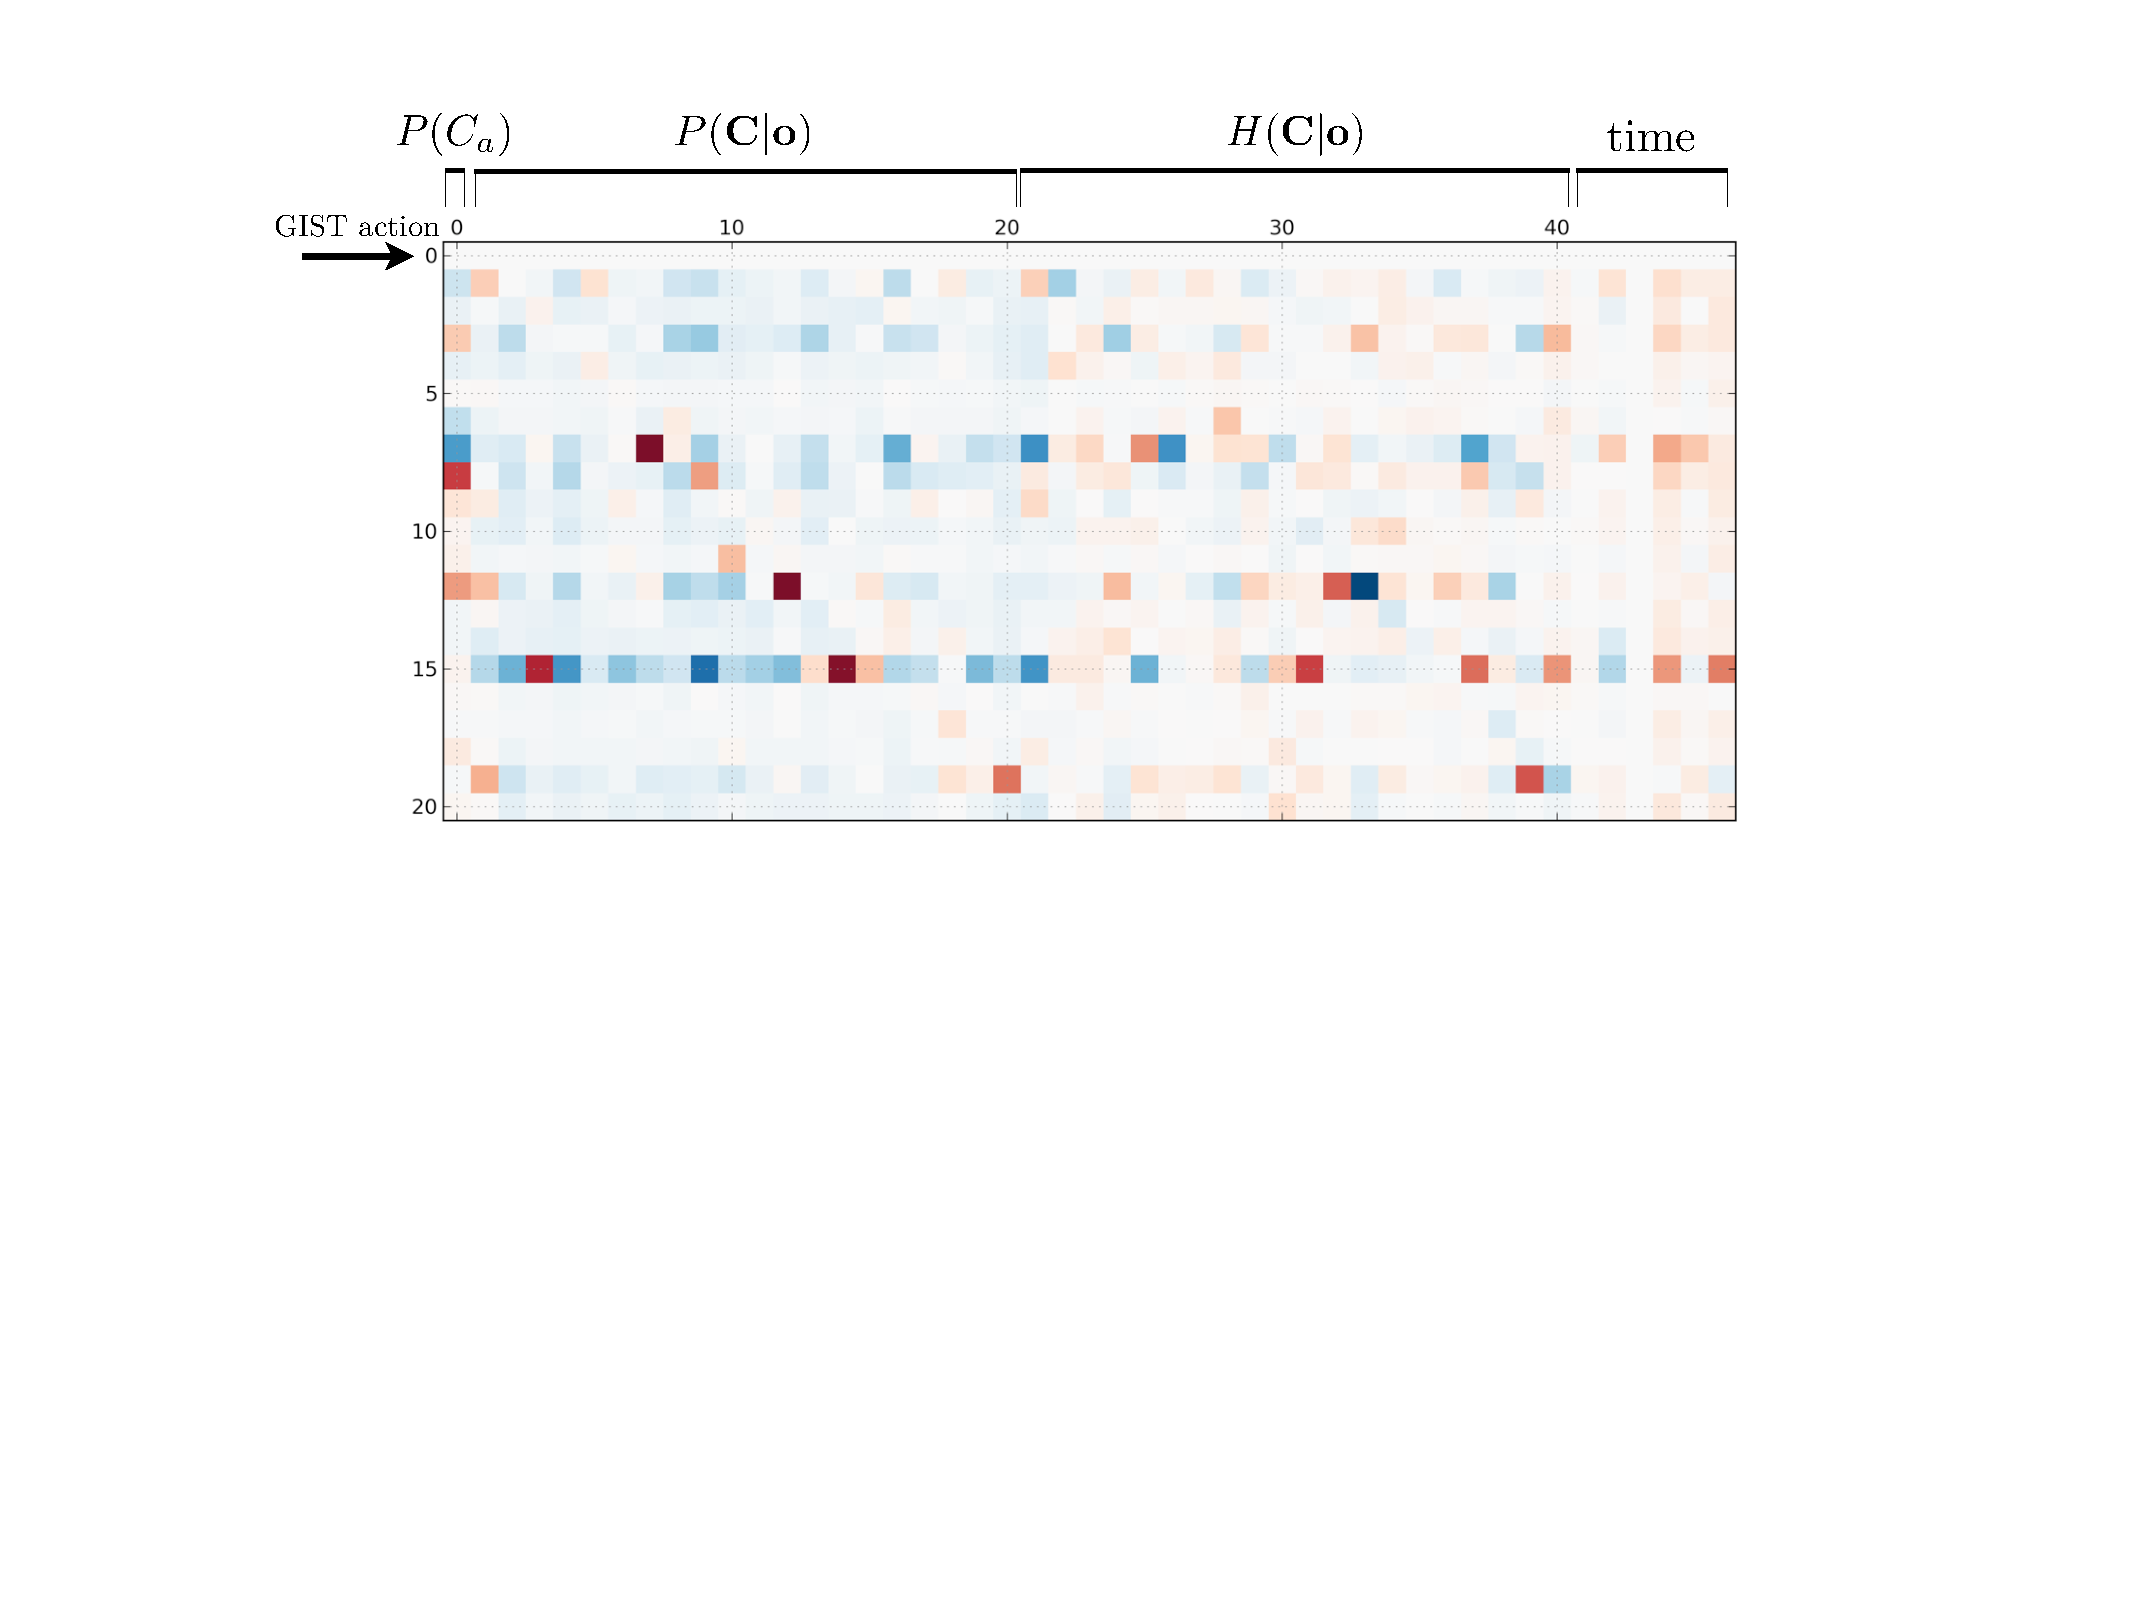
\includegraphics[width=0.49\linewidth]{../figures/weights_greedy}}
\subfloat[Reinforcement Learning]{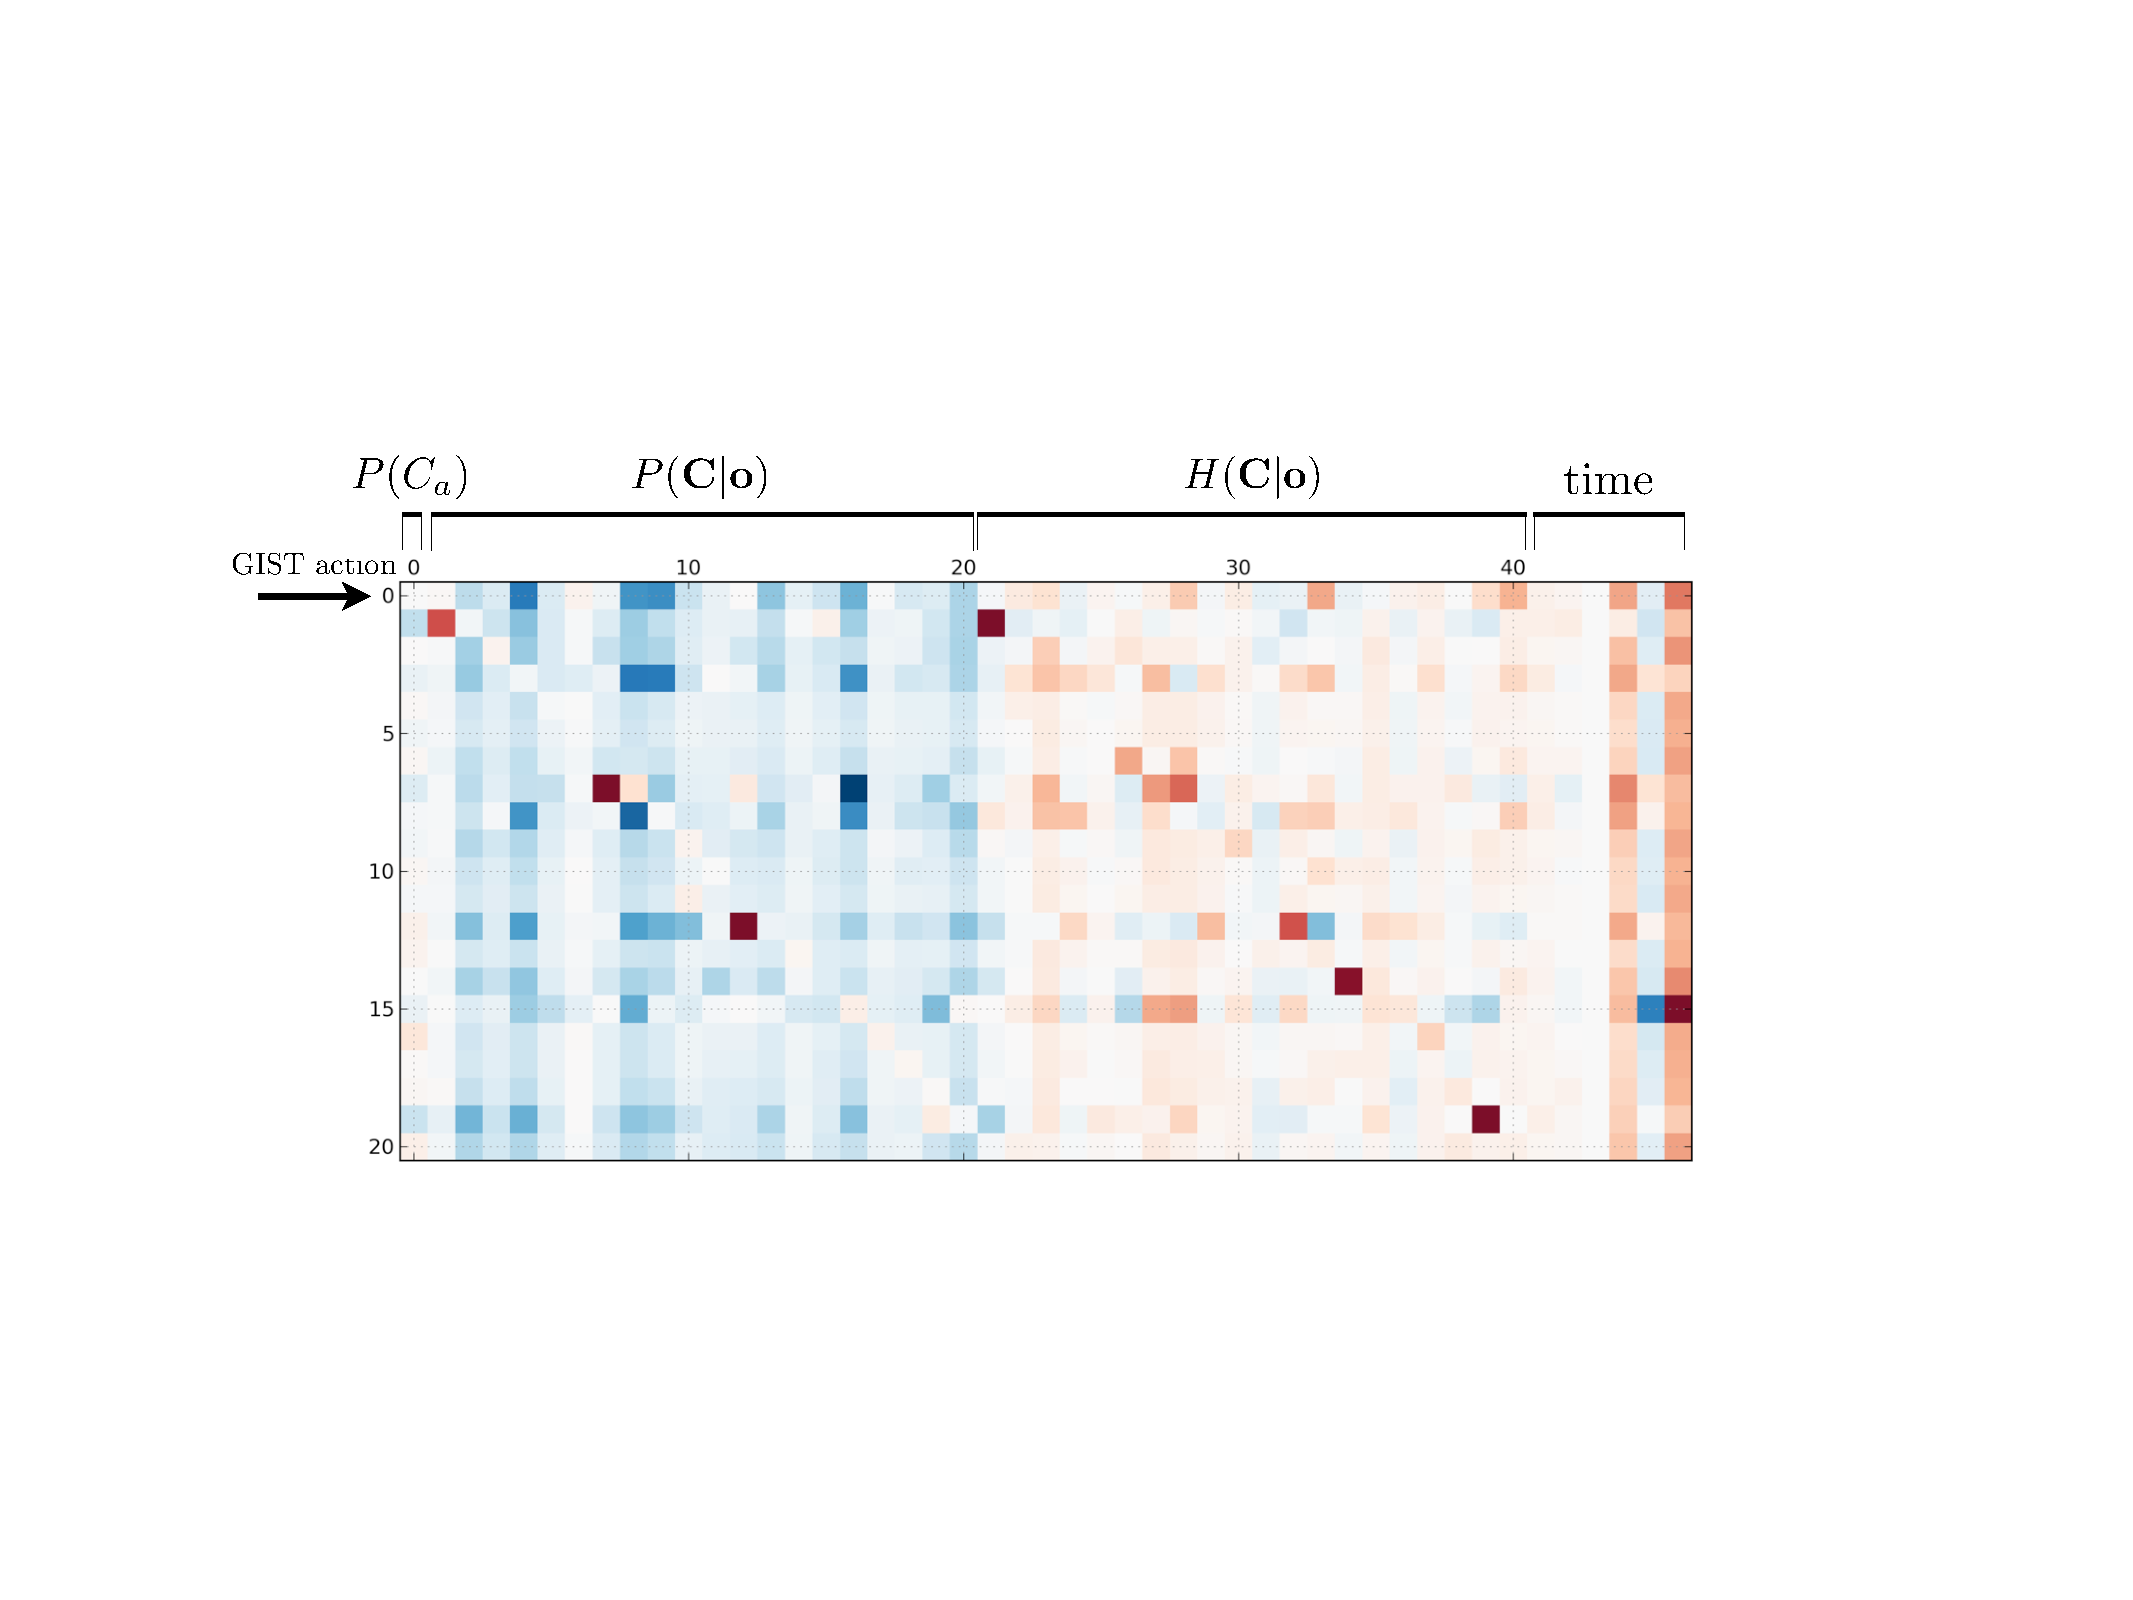
\includegraphics[width=0.49\linewidth]{../figures/weights_rl}}
% 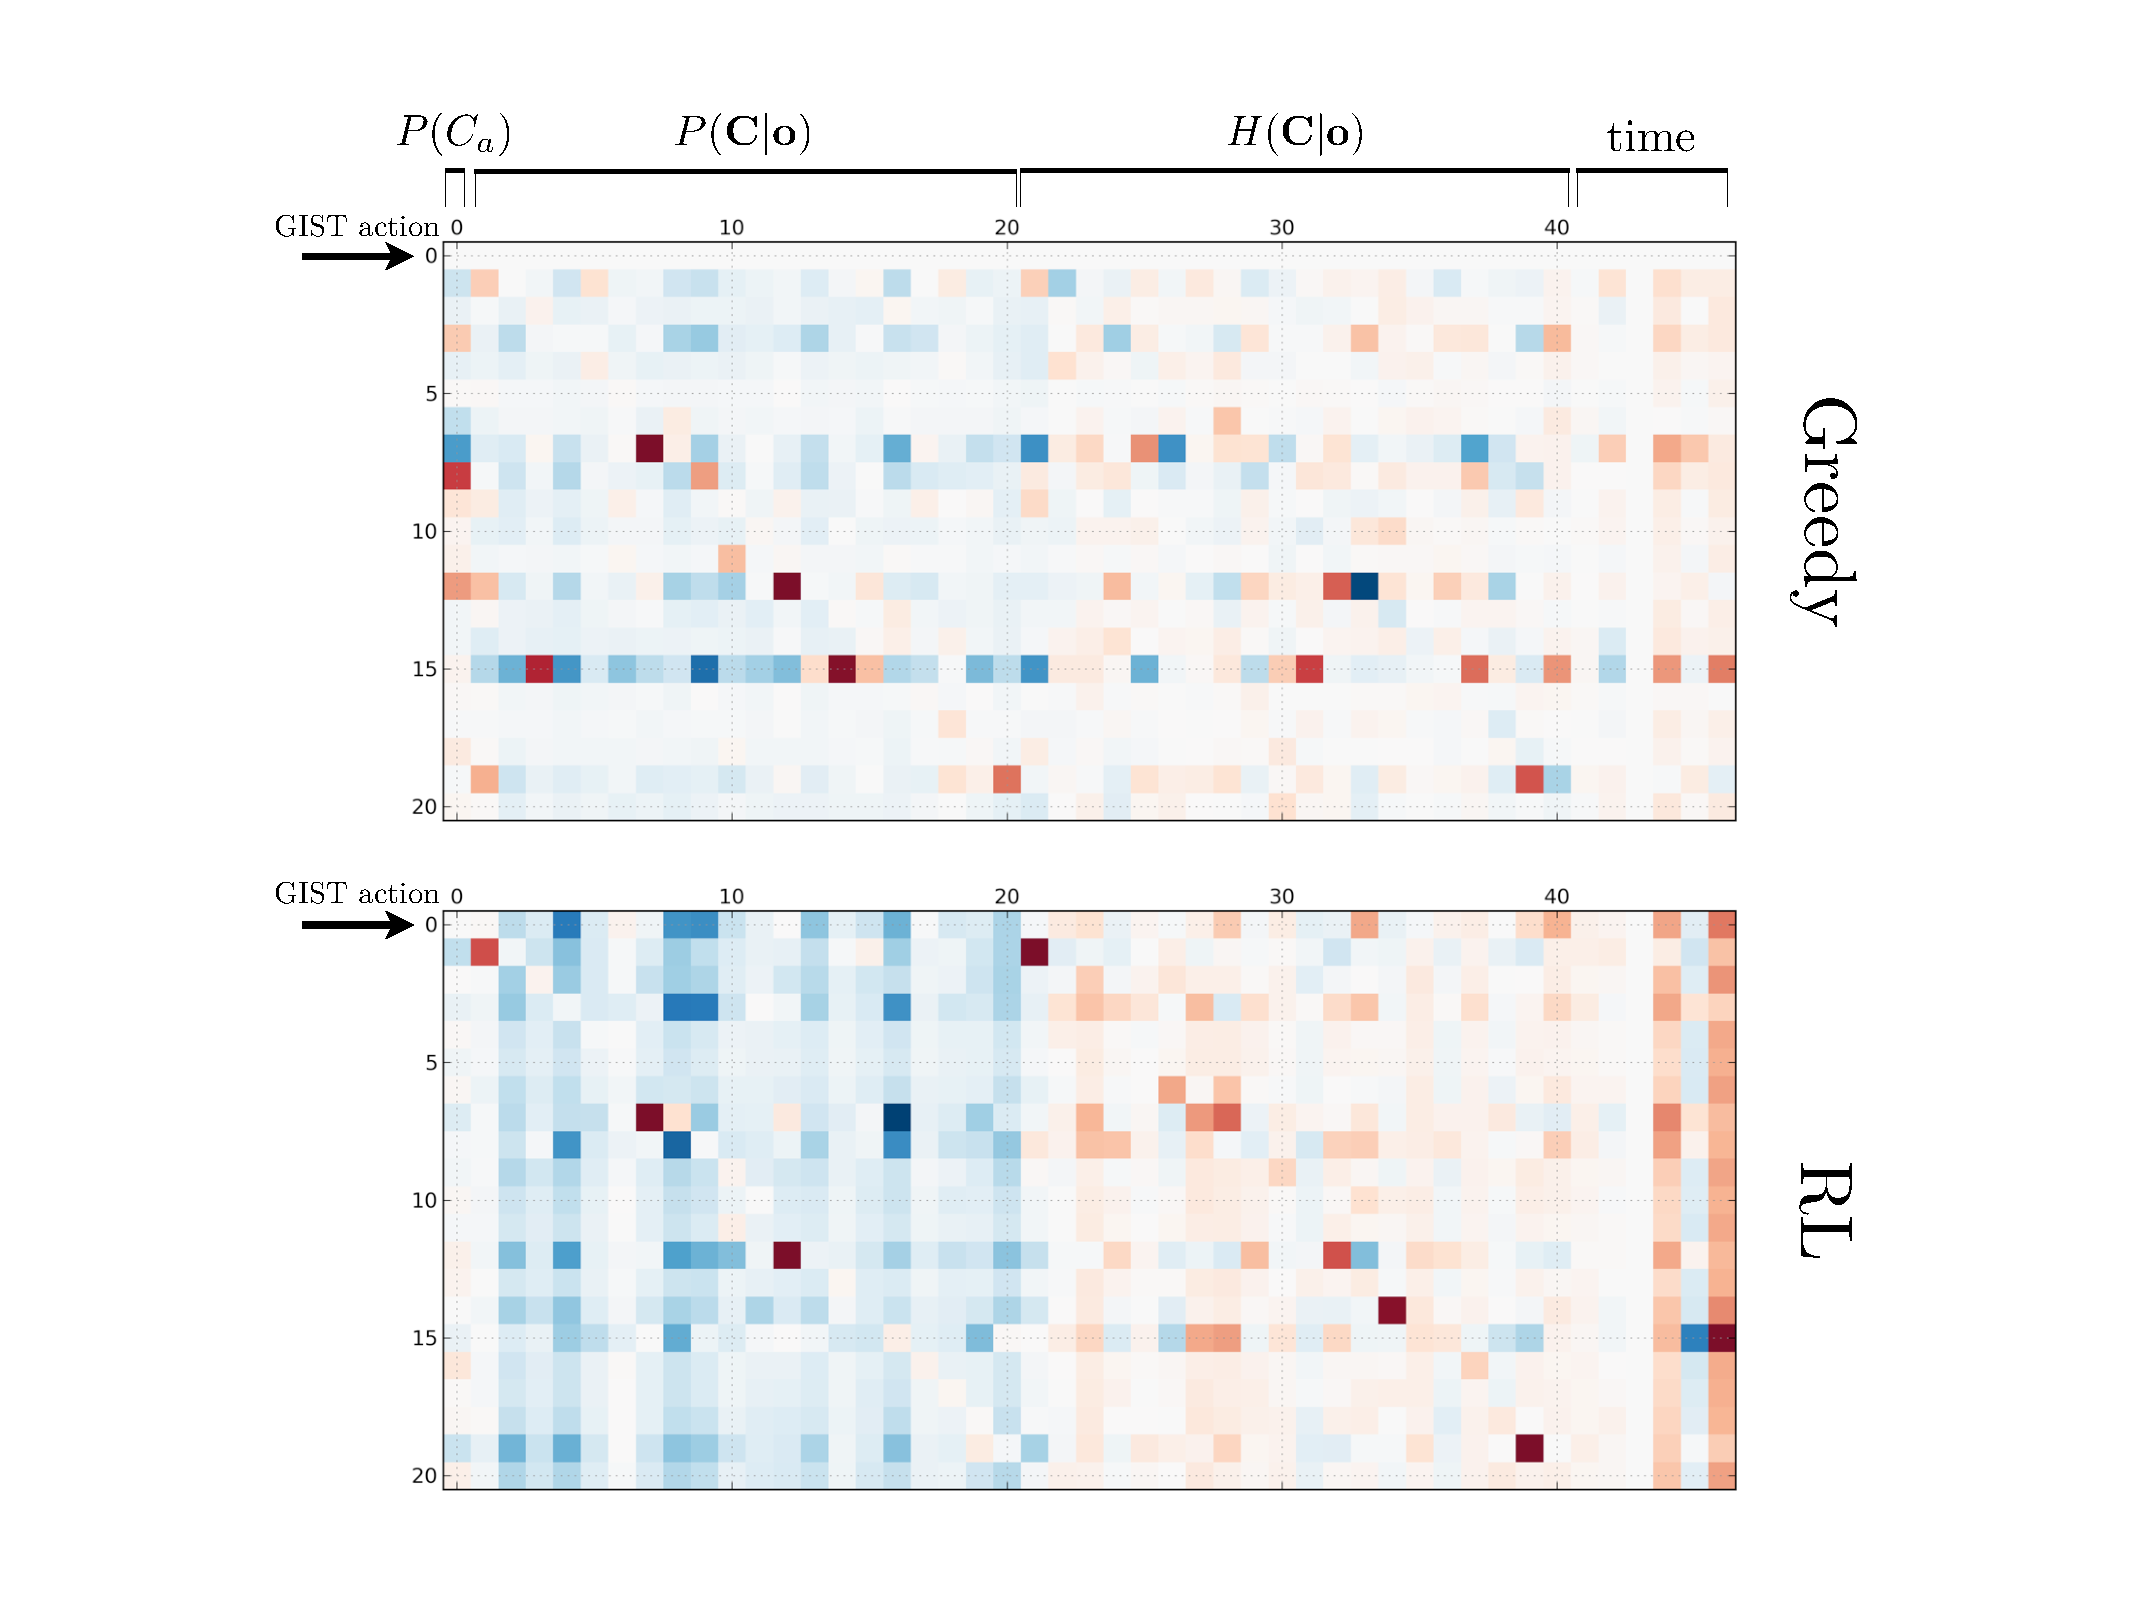
\includegraphics[width=0.87\linewidth]{../figures/weights.pdf}
\caption{
Learned policy weights $\theta_\pi$ (best viewed in color: red corresponds to positive, blue to negative values).
The first row corresponds to the scene-level action, which does not generate detections itself but only helps reduce uncertainty about the contents of the image.
Note that in the greedy learning case, this action is learned to never be taken, but it is shown to be useful in the reinforcement learning case.
}
\label{fig:weights}
\end{figure}

\subsection{Updating with observations} \label{sec:updating}

The bulk of our feature representation is formed by probability of individual class occurrence, conditioned on the observations so far: $P(C_0|\mathbf{o}) \ldots P(C_K|\mathbf{o})$.
This allows the action-value function to learn correlations between presence of different classes, and so the policy can look for the most probable classes given the observations.

However, higher-order co-occurrences are not well represented in this form.
Additionally, updating $P(C_i|\mathbf{o})$ presents choices regarding independence assumptions between the classes.
We evaluate two approaches for updating probabilities: \emph{direct} and \emph{MRF}.

In the \emph{direct} method, $P(C_i|\mathbf{o}) = score(C_i)$ if $\mathbf{o}$ includes the observations for class $C_i$ and $P(C_i|\mathbf{o}) = P(C_i)$ otherwise.
This means that an observation of class $i$ does not directly influence the estimated probability of any class but $C_i$.

The \emph{MRF} approach employs a pairwise fully-connected Markov Random Field (MRF), as shown in Figure~\ref{fig:figure1}, with the observation nodes set to $score(C_i)$ appropriately, or considered unobserved.

The graphical model structure is set as fully-connected, but some classes almost never co-occurr in our dataset.
Accordingly, the edge weights are learned with $L_1$ regularization, which obtains a sparse structure \cite{Lee2006}.
All parameters of the model are trained on fully-observed data, and Loopy Belief Propagation inference is implemented with an open-source graphical model package \cite{Jaimovich2010}.

An implementation detail: $score(C_i)$ for $a_{{det}_i}$ is obtained by training a probabilistic classifier on the list of detections, featurized by the top few confidence scores and the total number of detections.
Similarly, $score(C_i)$ for $a_{gist}$ is obtained by training probabilistic classifiers on the GIST feature, for all classes.

%!TEX root=../paper/paper.tex
\section{Evaluation}\label{sec:ccnn_evaluation}

\PM{Dataset}
We evaluate on the standard object detection benchmark: the PASCAL VOC \cite{pascal-voc-2010}.
In all cases, the CNN region classifiers are trained on the PASCAL VOC 2007 trainval set.
The parameters of our methods are set by training or cross-validation on the VOC 2007 val set.
We evaluate on the VOC 2007 test set.
The result plots and details are shown in \autoref{fig:voc2007_results} and \autoref{tab:ccnn_results}.

\PM{Implementation}
The scoring function for the quick-to-compute features is trained by a logistic regression classifier onto the max PASCAL overlap with any ground truth window on the validation dataset.
The classifier is optimized by stochastic gradient descent, and its regularization parameter is cross-validated.
The R-CNN software was used as available in June 2014.
\footnote{\url{https://github.com/rbgirshick/rcnn}}
That software relies on Selective Search \cite{Uijlings-IJCV-2013} region proposals.
Different images are proposed different numbers of regions.
\autoref{fig:roi_hist} shows the distribution of number of regions on the validation set, with the parameters of the R-CNN.
An additional parameter is the size of each batch of regions that goes through the CNN.
We set batch size to 100 regions, and observe that it takes on average 500 ms to process them with the CNN.
In all experiments, we use Ubuntu 12.04, Intel i5 3.2GHz CPU, and NVIDIA Tesla K40 GPU.

%!TEX root=../paper/paper.tex
\begin{figure}[ht]
\begin{subfigure}[b]{\linewidth}
    \centering
    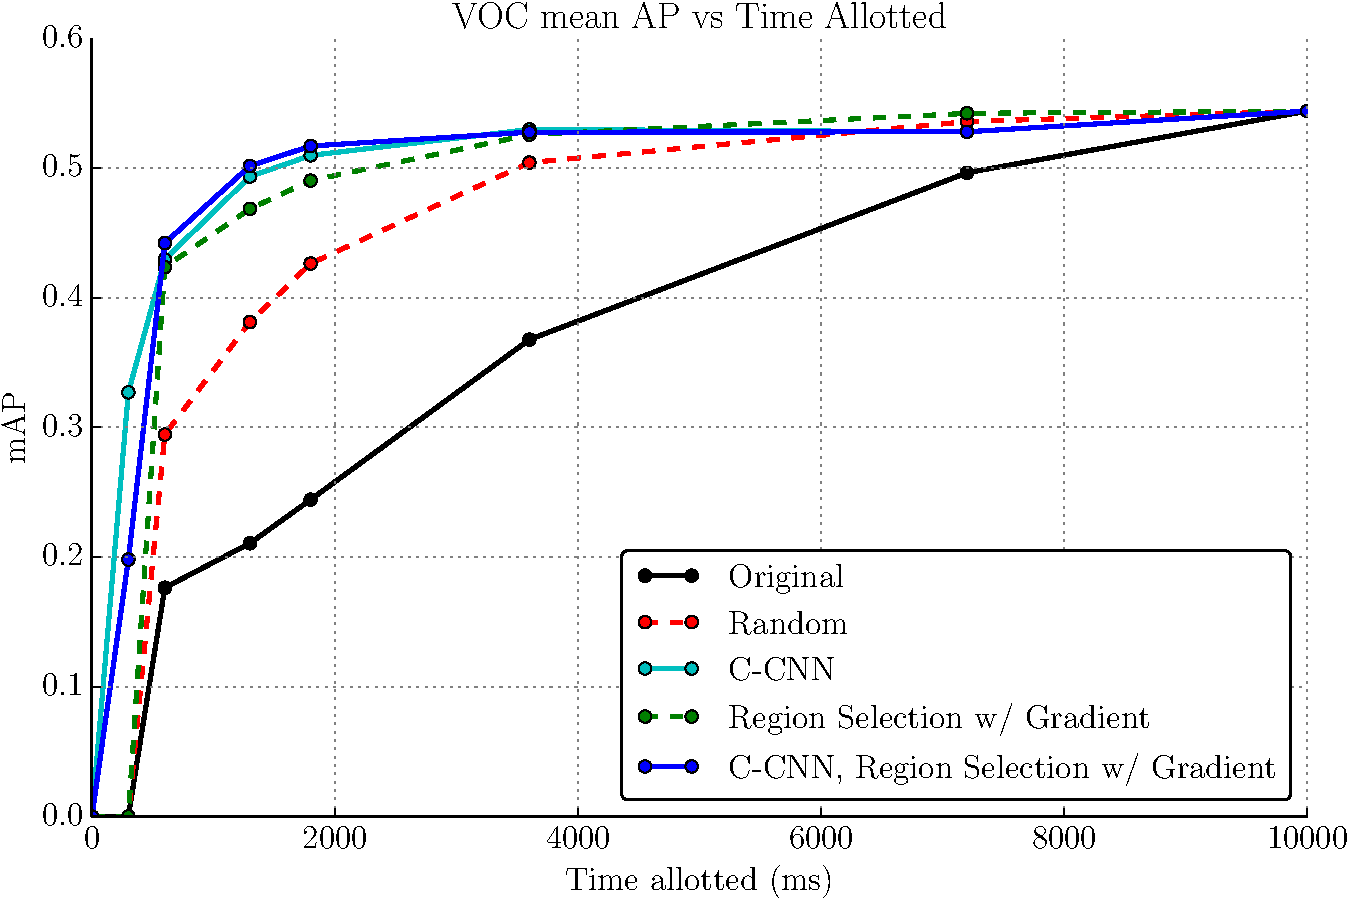
\includegraphics[width=.75\linewidth]{../ccnn/figures/_apvst_final.pdf}
    \caption{
Plotting Mean AP vs. Time Allotted allows comparison performance at a given time budget.
For example, at 1300 ms, random region selection gets about 0.42 mAP, while our best method (C-CNN with gradient-based region selection) obtains 0.50 mAP.
}\label{fig:apvst}
\end{subfigure}
\begin{subfigure}[b]{\linewidth}
    \centering
    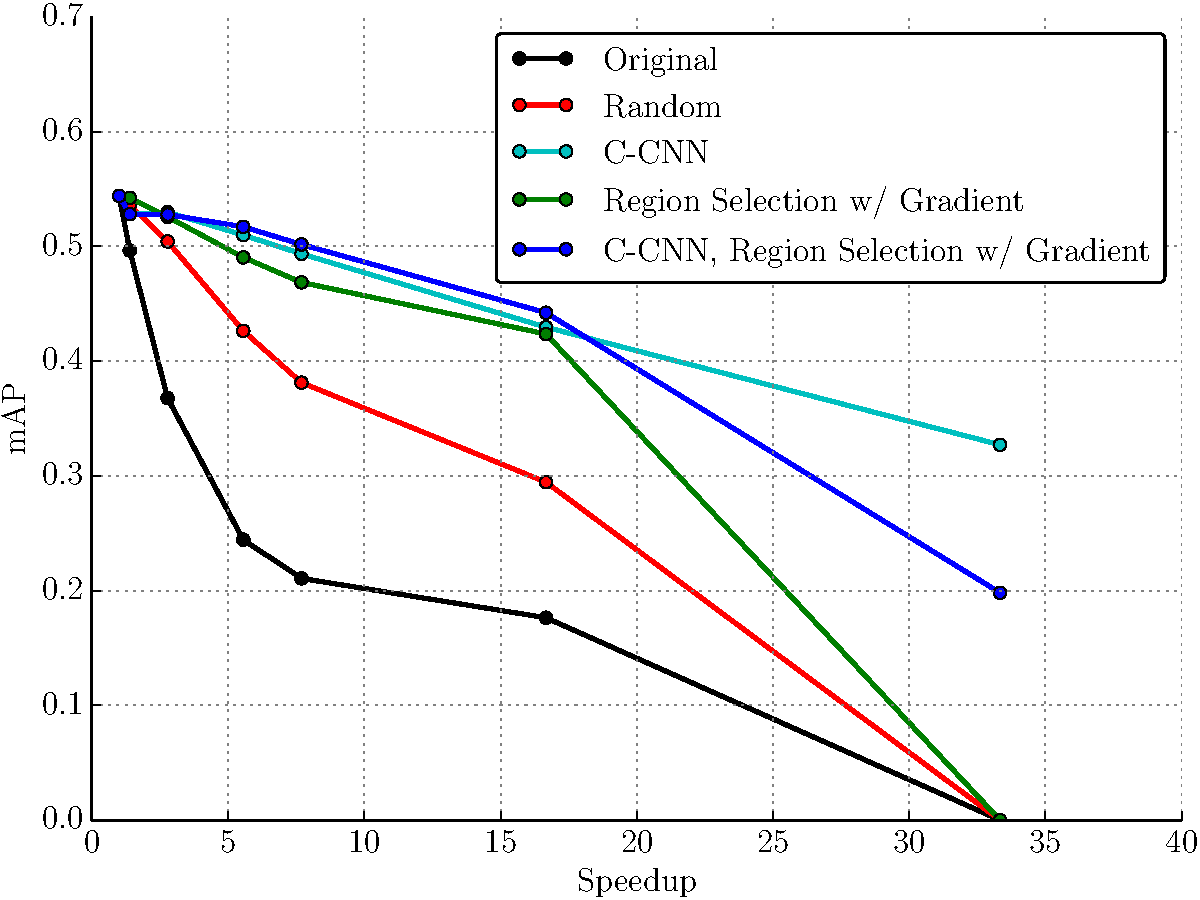
\includegraphics[width=.75\linewidth]{../ccnn/figures/_speedup_final_abs.pdf}
    \caption{
Plotting mean AP vs. speed-up factor allows comparison of speed-ups at a given mAP point.
For example, we can see that we should obtain mAP of 0.40 at around 20x speedup with our method.
}\label{fig:speedup}
\end{subfigure}
\caption{
Results of the Cascade CNN and other Anytime methods on the PASCAL VOC 2007 dataset.
}\label{fig:voc2007_results}
\end{figure}


\begin{table}[ht]
\centering
\caption{
Full table of AP vs. Time results on PASCAL VOC 2007.
Best performance for each time point is in bold.
}\label{tab:results}
\small{
\begin{tabular}{lrrrrrrrr}
\toprule
Time allotted (ms)                  & 0 & 300            & 600            & 1300           & 1800           & 3600           & 7200           & 10000 \\
\midrule
Original                            & 0 & 0.000          & 0.176          & 0.211          & 0.244          & 0.368          & 0.496          & 0.544 \\
Random                              & 0 & 0.000          & 0.295          & 0.381          & 0.426          & 0.504          & 0.536          & 0.544 \\
C-CNN                               & 0 & \textbf{0.327} & 0.430          & 0.493          & 0.510          & 0.528          & 0.528          & - \\
Region Selection w/ Gradient        & 0 & 0.000          & 0.424          & 0.469          & 0.490          & 0.526          & \textbf{0.542} & 0.544 \\
C-CNN, Region Selection w/ Gradient & 0 & 0.198          & \textbf{0.442} & \textbf{0.502} & \textbf{0.517} & \textbf{0.528} & 0.528          & - \\
\bottomrule
\end{tabular}
}
\end{table}


The experimental settings are
\begin{description}
  \item[Original] \hfill \\
  The original order of the Selective Search regions of interest.
  This order is influenced by the hierarchical segmentation of their method, and so has sequences of highly overlapping regions.

  \item[Random] \hfill \\
  A completely blind permutation of the original order.

  \item[Region Selection] \hfill \\
  The region statistics feature is always used.
  Additionally, we consider the Pixel Gradient feature, with \emph{setup time} of the gradient forward-back propagation of 20 ms.

  \item[Cascaded CNN] \hfill \\
  The Cascaded CNN model, as described in \autoref{sec:ccnn}.
  The first experiment (C-CNN) takes batches of regions in a random order.
  The next two experiments also make use of the Region Selection methodology with the quick-to-compute feature.
\end{description}

\PM{Analysis}
Since the time to process a full batch with a non-cascaded CNN is 500 ms, there are no results for non-cascaded baselines at 300 ms.
At this time, the Cascaded CNN without any region ordering is best.
A reason for why C-CNN with Region Selection is not as good at this point is that the region selection presents better region candidates, with fewer rejection opportunities, and thus has less coverage of the image.
At 600 ms, C-CNN method have had more than one batch go through, and the Region Selection is giving it a lead over the simple C-CNN.
Both method are better than the baseline non-cascaded methods for this entire duration.

% !TEX root = paper/paper.tex
\section{Related Work}
% \paragraph{Feature combination and selection.}
% \emph{Boosting} is a method for combining weak learners into a more powerful classifier \cite{Hastie2009}.
% A popular use of boosting is in introducing non-linearities by training depth-limited decision trees as weak learners---the boosting trick.
% For SVM-based classifiers, \emph{Multiple Kernel Learning} (MKL) provides a way to train classifiers using an automatically weighted combination of kernels \cite{Lanckriet2004}.
% It has been shown that MKL is outperformed by boosting single-kernel classifiers \cite{Gehler2009}.
% Of course, if all classifiers are linear, then combining outputs of classifiers trained on different feature channel with another classifier is equivalent to training one classifier on all features at once.
% \todo{What about learning a \emph{non-linear} second classifier on top of the weak learner scores---any papers?}

% \todo{A couple of sentences on feature selection approaches, particularly using infogain as proxy for classification error.}

\paragraph{Static selection}% test-time efficient feature selection.}
% The simplest way to limit the number of features used at test time is to $L_1$-regularize.
% This method does not explicitly consider feature cost, nor is it able to evaluate features one by one, or to give an answer before all features are computed.

A well-known method to evaluate features sequentially is the cascaded boosted classifier of Viola \& Jones \cite{Viola2004} (updated by Bourdev \& Brandt \cite{Bourdev-CVPR-2005} with a soft threshold), which is able to quit evaluating an instance before all features are computed---but feature cost was not considered.
The cost-sensitive cascade of Chen et al.\ \cite{Chen-AISTATS-2012} optimizes stage order and thresholds to jointly minimize classification error and feature computation cost.
Xu et al.\ \cite{Xu-ICML-2012} and Grubb \& Bagnell \cite{Grubb-AISTATS-2012} separately develop a variant of gradient boosting for training cost-sensitive classifiers; the latter prove near-optimality of their greedy algorithm with submodularity results.
Their methods are tightly coupled to the stage-wise regression algorithm.

\vspace{-1em}
\paragraph{Dynamic selection}% test-time efficient feature selection.}
The above methods learn an efficient but \emph{fixed} order for evaluating features given a test instance.

Gao \& Koller \cite{Gao-NIPS-2011} propose a method for \emph{active classification}: myopically selecting the next feature based on expected information gain given the values of the already selected features.
The method is based on locally weighted regression, highly costly at test time.
Ji \& Carin \cite{Ji-PR-2007} also formulate cost-sensitive feature selection generatively, as an HMM conditioned on actions, but select actions myopically, again at signficant test time cost.

Karayev at al.\ \cite{Karayev-NIPS-2012} propose a reinforcement learning approach for selecting object detectors; they rely on expensive test-time inference in a graphical model to combine observations.
Dulac-Arnold et al.\ \cite{Dulac-Arnold-ML-2012} present another MDP-based solution to ``datum-wise classification'', with an action space comprised of all features and labels, recently extended to region-based processing \cite{Dulac-Arnold-ICLR-2014}.
He He et al.\ \cite{HeHe-ICMLW-2012} also formulate an MDP with features and a single classification step as actions, but solve it via imitation learning of a greedy policy.
Benbouzid et al.\ \cite{Benbouzid-ICML-2012} formulate an MDP that simply extends the traditional sequential boosted classifier with an additional \emph{skip} action, significantly limiting the space of learnable policies (\cite{Trapeznikov} provides another variation on this problem).
Although \cite{Karayev-NIPS-2012} targets \emph{Anytime} performance, their inference procedure is prohibitively expensive for test-time use in a general classification task.
In contrast, our fast linear method allows direct specification of the Anytime cost budget.

\emph{Label trees} also guide an instance through a tree of classifiers; their structure is determined by the confusion matrix or learned jointly with weights \cite{Deng-NIPS-2011}.
Xu et al.\ \cite{Xu-ICML-2013} learn a cost-sensitive binary tree of weak learners using an approach similar to the cyclic optimization of \cite{Chen-AISTATS-2012}.
Less directly related---but exciting for its novelty---is the work of \cite{weiss2013dynamic}, who apply simple introspection to structured models for a significant speedup of human pose estimation.
Another exciting direction is theoretical analysis of near-optimal policies with humans in the loop \cite{chen14active}.


\bibliographystyle{splncs}
\bibliography{sergeyk-bibtex,misc}

\end{document}
